%*******************************************************************************
%*******************************************************************************
\chapter{Songbook}
\setcounter{chapter}{1}
\label{chap:songbook}
\minitoc
\fancyhead[RE]{\textit{Chapitre \arabic{chapter}.~\nouppercase{\leftmark}}}
\fancyhead[LO]{\textit{\arabic{chapter}.\arabic{section}.~\nouppercase{\rightmark}}}
%*******************************************************************************
%*******************************************************************************


%*******************************************************************************
\section{Installation}
\label{sec:install}
%*******************************************************************************

De manière générale, évitez les chemins contenant des espaces ou des
caractères spéciaux. Dans ce manuel, le répertoire de travail est
supposé être~: \directory{\$HOME/songbook} pouvant être noté
\directory{/home/user/songbook} ou \directory{$\sim$/songbook}.

Le songbook utilise \LaTeX{} pour la mise en page des chansons et
Python pour la génération des tables des matières (dépendances
obligatoires). Il est également possible d'inclure en option des
partitions générées avec Lilypond (dépendances recommandées). Enfin,
vous aurez besoin d'un logiciel pour lire les fichiers \ext{pdf}
produits.

%------------------------------------------------------------------------------
\subsection{\linux}
%------------------------------------------------------------------------------

\paragraph{Dépendances}

Installation des dépendances obligatoires.
\begin{unix}
  sudo apt-get install texlive-base texlive-latex-extra
  sudo apt-get install texlive-lang-french python
\end{unix}

Installation des dépendances recommandées.
\begin{unix}
  sudo apt-get install texlive-fonts-recommended
  sudo apt-get install texlive-fonts-extra
  sudo apt-get install lilypond
\end{unix}

\paragraph{Téléchargement des sources}

Les sources peuvent être récupérées sous la forme d'une archive \ext{tar.gz}
\begin{unix}
  wget http://www.patacrep.com/data/documents/songbook.tar.gz
  tar xzvf songbook.tar.gz
\end{unix}

ou sous la forme d'un dépôt \git

\begin{unix}
  git clone git://git.lohrun.net/songbook.git
\end{unix}

\paragraph{Exécution}

Un \emph{makefile} automatise tout le processus de compilation. 
Dans le répertoire du songbook~:

\begin{unix}
  make all
\end{unix}

Quelques options de base du makefile~:
\begin{itemize}
\item \command{\$ make clean}~: supprime tous les fichiers de logs et
  les fichiers générés à part les recueils finaux \ext{pdf}.
\item \command{\$ make cleanall}~: supprime tous les fichiers générés,
  y compris les PDF.
\item \command{\$ make lilypond}~: génère dans \directory{./lilypond} les
  PDF de toutes les partitions lilypond \ext{ly} trouvées dans
  \directory{./lilypond}. Il est nécessaire d'avoir installé
  \emph{lilypond} au préalable.
\item \command{\$ make archive}~: crée une archive compressée
  \file{songbook.tar.gz} des fichiers sources du projet.
\item \command{\$ make book.pdf}~: la compilation de tous les carnets
  pouvant être longue, si seule une version précise vous intéresse,
  vous pouvez lancer la compilation d'un seul fichier \ext{pdf}. À la place
  de \file{book.pdf}, vous pouvez utiliser~:
\end{itemize}

\begin{center}
  \begin{tabular}{l l}
    \hline
    \command{make} & description \\
    \hline
    \file{songbook.pdf} &~: version complète avec toutes les chansons \\
    \file{volume-$i$.pdf} &~: crée le volume $i$ (environ 160 pages)\\
    \file{naheulbeuk.pdf} &~: version spéciale Donjon de Naheulbeuk\\
    \file{english.pdf} &~: chansons en anglais uniquement\\
    \file{french.pdf} &~: chansons en français uniquement\\
    \hline
  \end{tabular}
\end{center}

La commande \command{make} sans option correspond à \command{make
  \file{songbook.pdf}}.

%------------------------------------------------------------------------------
\subsection{\windows}
%------------------------------------------------------------------------------

\paragraph{Dépendances}

Installation des dépendances obligatoires.
\begin{itemize}
\item Miktex~: \url{http://miktex.org/}
\item Python~: \url{http://www.python.org/download/releases/2.7.3/}
\end{itemize}

\begin{nota}
La compilation sous \windows a uniquement été testée avec~: MikTeX~2.9
et Python~2.7.3.
\end{nota}

Installation des dépendances recommandées.
\begin{itemize} 
\item Lilypond~: \url{http://lilypond.org/install/}
\end{itemize}


\paragraph{Modification de la variable \command{Path}}

Il faut maintenant modifier la variable \command{Path} de votre
système.
\begin{itemize}
\item Clic-droit sur Poste de travail (XP) ou sur Ordinateur (Vista,
  Seven) puis Propriétés.
\item Dans \menu{Paramètres}{Système Avancés}, cliquez sur Variables
  d'environnement.
\end{itemize}

Dans la partie basse (Variables système), faîtes dérouler la liste
jusqu'à trouver \command{Path}. La variable est modifiable en
double-cliquant dessus. Le \command{Path} contient un ensemble de
chemins séparés par des \emph{points-virgules}. Assurez-vous qu'elle
contient les chemins suivants. Dans le cas contraire, ajoutez-les~:
\begin{itemize}
\item Python~: \verb#C:\Python27#
\item Miktex~: \verb# C:\Program Files\MiKTeX 2.9\miktex\bin#
\item Lilypond~: \verb#C:\Program Files\LilyPond\usr\bin#
\end{itemize}                     

\begin{nota}
Attention aux numéros de version. Ces répertoires sont donnés à titre
indicatifs et peuvent être légèrement différents suivant la version
que vous aurez téléchargée.
\end{nota}

Redémarrez votre ordinateur après avoir modifié la variable
\command{Path}.


\paragraph{Téléchargement des sources}

Les sources peuvent être récupérées sous la forme d'une archive
\ext{tar.gz} à l'adresse~:
\url{http://www.patacrep.com/data/documents/songbook.tar.gz}. Vous
pouvez en extraire le contenu à l'aide de logiciels comme
7zip\footnote{\url{http://www.7-zip.org/}} ou
Winrar\footnote{\url{http://www.win-rar.com/}}.

Alternativement, si vous avez installé un client
Git\footnote{\url{http://git-scm.com/}} sur votre machine, par exemple
Mysysgit\footnote{\url{http://code.google.com/p/msysgit/}}, vous
pouvez utiliser l'adresse suivante pour récupérer les sources~:

\begin{unix}
  git clone git://git.lohrun.net/songbook.git
\end{unix}

\paragraph{Exécution}

\begin{enumerate}
\item Ouvrez l'invite de commandes \windows~: \Key{Windows}+\Key{r}, entrez
  \command{cmd} et validez par \Key{Entrée}
  (\reffig{fig:terminal-windows}).
\item Allez dans le répertoire du songbook en utilisant la commande \command{cd}.
Par exemple,
  \begin{unix}
    cd C:\
    cd songbook
  \end{unix}
\item Utilisez l'exécutable \file{make.bat} en donnant en paramètre un fichier \ext{sb}.
  Par exemple,
  \begin{unix}
    make.bat songbook.sb
  \end{unix}
\end{enumerate}

\begin{nota}
MikTeX est une distribution \LaTeX{} qui permet d'installer {\og}à la
volée{\fg} les \emph{paquets} manquants. Installez les paquets requis
(\reffig{fig:paquets-miktex}).
\end{nota}

%*******************************************************************************
\section{Description du contenu}
\label{sec:contents}
%*******************************************************************************

\paragraph{\directory{./utils}}
\label{sec:utils}
Contient un ensemble de scripts utilitaires. Un script s'exécute par la commande~:

\begin{unix}
  ./utils/script.sh
\end{unix}

\begin{itemize}
\item \file{resize-cover.sh}~: permet de redimensionner
  automatiquement tous les fichiers \ext{jpg} du répertoire
  \directory{songbook/songs} correspondant aux pochettes des albums. À
  exécuter après l'ajout d'une nouvelle pochette jpg.

\item \file{rules.py}~: applique un ensemble de règles
  automatiques pour les notations \LaTeX{} de certains caractères et
  pour les notations d'accords. À exécuter après l'ajout d'une
  nouvelle chanson pour être sûr de respecter les standards du
  songbook.

\item \file{new-songs-list.sh}~: permet de récupérer la liste des
  chansons ajoutées depuis la dernière version.

\item \file{make-html.sh}~: génère la liste de toutes les chansons au
  format html.
\end{itemize}

\paragraph{\directory{./templates}}
Contient les fichiers de style du songbook et permet de modifier des
paramètres comme la police utilisée, les différentes couleurs
utilisées etc.

\begin{itemize}
\item \file{patacrep.tmpl}~: template par défaut correspondant à la
  mise en page classique.
\item \file{patacrep-en.tmpl}~: version traduite en anglais du
  template par défaut.
\item \file{minimal.tmpl}~: une version plus compacte sans page de
  garde ni table des matières.
\end{itemize}

%%%%%%%%%%%%%%%%%%%%%%%%%%%%%% FIGURE %%%%%%%%%%%%%%%%%%%%%%%%%%%%%%%%%%
\begin{figure}
  \centering
  %% -- subfigures --
  \subfigure[]{
    \label{fig:templates-a}
    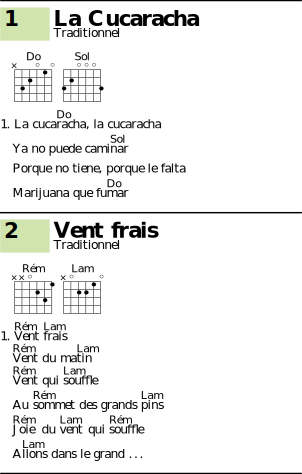
\includegraphics[width=0.35\textwidth]{templates-a}%
  }%
  \hspace{0.1cm}%
  \subfigure[]{%
    \label{fig:templates-b}%
    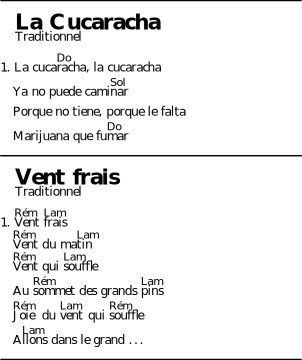
\includegraphics[width=0.35\textwidth]{templates-b}%
  }%
  %% -- subfigures --
  \caption[Templates]{% 
    Différents modèles de document peuvent être utilisés.
    \subref{fig:templates-a}~Template \file{patacrep.tmpl}; % 
    \subref{fig:templates-b}~Template \file{minimal.tmpl}.%
  }%
  \label{fig:templates}
\end{figure}
%%%%%%%%%%%%%%%%%%%%%%%%%%%%%%%%%%%%%%%%%%%%%%%%%%%%%%%%%%%%%%%%%%%%%%%%


\paragraph{\directory{./songs}}
Contient l'ensemble des chansons disponibles sous la forme de fichiers
\ext{sg}. Chaque chanson se trouve dans un sous-répertoire du nom
de l'artiste. Par exemple~:
\file{songs/Pornophonique/Sad\_robot.sg}.

\paragraph{\directory{./lilypond}}
Contient les sources des partitions Lilypond sous la forme de fichiers
\ext{ly}.

\paragraph{\directory{./tex}}
Contient différents fichiers \LaTeX{} (licences etc.).

\paragraph{\directory{./books}}
Contient les fichiers \ext{sb} qui correspondent aux différents
recueils PDF mis à disposition sur \url{www.patacrep.com}.

\paragraph{\directory{./covers}}
Répertoire temporaire contenant les pochettes des albumes. Ce
répertoire est généré automatiquement lors de la compilation d'un
recueil et est uniquement présent pour des raisons de performance.

\paragraph{\directory{./img}}
Contient les images utilisées dans les songbooks (exceptés les
pochettes des albums). Pour rajouter \file{mon\_image.jpg} dans une
chanson, utilisez la macro \latexcom{image} dans un fichier
\ext{sg}. Cette macro se comporte comme la commande \LaTeX{}
\latexcom{includegraphics}. Par exemple~:

\begin{songbook}
  \image[width=4cm]{mon_image}
\end{songbook}

%*******************************************************************************
\section{Créer un recueil}
\label{sec:create-songbook}
%*******************************************************************************

Pour produire un recueil, vous devez créer un fichier \ext{sb} dont le
contenu est précisé ci-après. Les fichiers songbook \ext{sb}
contiennent un ensemble d'options pour la personnalisation du recueil
ainsi qu'une liste de chansons. Ces recueils doivent être enregistrés
dans le répertoire \directory{./books}.

\begin{code}
{
"template" : "minimal.tmpl",
"bookoptions" : [
    "diagram",
    "lilypond",
    "pictures"
  ],
"songs" : [
    "Le_Donjon_de_Naheulbeuk/10_sous_dans_ma_poche.sg",
    "Le_Donjon_de_Naheulbeuk/Bugger_off.sg"
  ]
}
\end{code}

Les options disponibles sont présentes dans le fichier \ext{tmpl}
utilisé. Dans le cas du template \file{patacrep.tmpl}, les options
disponibles sont les suivantes~:

\begin{center}
  \rowcolors{1}{white}{Aluminium1}
  \begin{tabular}{l l l}
    \hline\noalign{\smallskip}
    Option & Description  & Type \\
    \noalign{\smallskip}
    \hline
    \noalign{\smallskip} 
    title & le titre du recueil & chaîne de caractères \\
    author & l'auteur du recueil & chaîne de caractères \\
    booktype & avec ou sans accords & \command{chorded} ou \command{lyric}\\
    lang & langue du recueil & \command{french}, \command{english}, etc. \\
    instruments & instruments à afficher & \command{guitar}, \command{ukulele} \\
    bookoptions & affichage des éléments & \command{lilypond}, \command{diagram},\\
    & & \command{importantdiagramonly},\\
    & & \command{onesongperpage}, \command{pictures},\\
    & & \command{repeatchords}, \command{tabs}\\
    version & la version actuelle du PDF & chaîne de caractères \\
    subtitle & sous-titre du recueil & chaîne de caractères \\
    web & adresse de votre site & chaîne de caractères \\
    mail & votre adresse email & chaîne de caractères \\
    picture & l'image de la page de garde & chemin vers image\\
    & & \ext{png}, \ext{jpg} ou \ext{pdf}\\
    picturecopyright & copyright de l'image & chaîne de caractères \\
    footer & pied de page & chaîne de caractères \\
    license & licence du document & chaîne de caractères \\
    mainfontsize & taille de la police & 10, 11 ou 12\\
    songnumberbgcolor & couleur des numéros des chansons & code hexadécimal \\
    notebgcolor & couleur des notes dans les chansons & code hexadécimal \\
    indexbgcolor & couleur des liens dans l'index & code hexadécimal \\
    \hline
  \end{tabular}
\end{center}

Description des \og bookoptions \fg{} :
\begin{description}
  \item[\command{diagram}] affiche les diagrammes des accords ;
  \item[\command{importantdiagramonly}] affiche les diagrammes des
    accords, mais seulement ceux marqués comme important par le
    transcripteur de la chanson ;
  \item[\command{lilypond}] affiche les partitions Lilypond ;
  \item[\command{pictures}] affiche les couvertures des albums ;
  \item[\command{tabs}] affiche les tablatures ;
  \item[\command{repeatchords}] répète les accords dans tous les
    couplets des chansons, si la transcription le permet ;
  \item[\command{onesongperpage}] force l'affichage d'une seule
    chanson par page.
\end{description}

Pour compiler votre recueil \file{mybook.sb}~:
\begin{unix}
make mybook.pdf
\end{unix}


%*******************************************************************************
\section{Écrire une chanson}
\label{sec:write-song}
%*******************************************************************************

%------------------------------------------------------------------------------
\subsection{Éléments principaux}
%------------------------------------------------------------------------------

Une chanson est un fichier texte \file{chanson.sg} placé dans
le répertoire \directory{songs/Artiste}. Les espaces n'étant pas
tolérées, veillez à utiliser des tirets bas (\emph{underscores}.
L'en-tête d'un fichier
\ext{sg} se présente de la manière suivante~:

\begin{songbook}
\beginsong{Titre}
  [by=<Artiste>,cov=<album-cover>,album=<Album>]
\end{songbook}

Les paramètres \command{Titre}, \command{Artiste},
\command{album-cover} et \command{Album} sont à renseigner pour chaque
nouvelle chanson. Le paramètre \command{album-cover} désigne un
fichier \file{album-cover.jpg} devant se trouver dans le même
répertoire que le fichier \ext{sg}.

La chanson se compose d'une succession de couplets \anglais{verse} et
de refrains \anglais{chorus}. Un couplet figure dans un environnement
\command{verse}, c'est-à-dire qu'il commence par \verb|\begin{verse}|
et se termine par \verb|\end{verse}|. De la même manière, un refrain
est placé dans un environnement \command{chorus}, c'est-à-dire entre les
balises \verb|\begin{chorus}| et \verb|\end{chorus}|. Les paroles sont
écrites normalement entre les balises d'ouverture et de fermeture de
l'environnement.

Pour préciser sur quelle syllabe un accord doit être joué, on utilise
une commande spéciale. Par exemple, la commande \latexcom{[E]}
produira un \command{Mi} au dessus de la syllabe suivante dans le PDF.

\begin{songbook}
\begin{verse}
  His \[Dm]steely skin is covered
  By \[F]centuries of dust
  \[C]Once he was a great one
  \[Dm]Now he's dull and rust
\end{verse}
\end{songbook}

Chaque chanson se termine avec la commande \latexcom{endsong}.

%------------------------------------------------------------------------------
\subsection{Règles de style}
%------------------------------------------------------------------------------

De nombreuses règles de style peuvent être appliquées automatiquement
à l'ensemble des chansons via le script \file{utils/rules.py}. Ce
script vérifie les espaces en fin de ligne, certaines règles de
ponctuation, quelques fautes d'orthographe etc. Pour l'utiliser,
exécutez la commande suivante dans le répertoire du songbook :

\begin{unix}
python utils/rules.py
\end{unix}

\paragraph{Notation des accords}
Il est impératif d'utiliser la convention anglo-saxone de notation des
accords (A, B, C, D, E, F, G) et non pas la notation latine (La, Si,
Do, Ré, Mi, Fa, Sol). En revanche, suivant suivant le paramètre
\emph{langue} du template utilisé, le rendu des accords dans le PDF
pourra être différent (l'accord \latexcom{[D]} sera affiché
\command{Ré} si la langue du songbook est \emph{french}).

Par défaut, l'accord est majeur (C fait référence à l'accord de Do
majeur). Les accords mineurs sont précisés par un \command{m}
minuscule.  Le symbole bémol $\flat$ est représenté en utilisant le
caractère \command{\&}. Le dièse $\sharp$ est codé par le caractère
\command{\#}. Les autres notations sont simplement ajoutées comme des
caractères à l'accord principal. Par exemple, l'accord de \command{La
  bémol mineur} est noté \latexcom{[A\&m]}.

\begin{nota}
  Pour des raisons techniques, le symbole \command{\#} ne peut pas
  être utilisé dans les environnements \latexcom{nolyrics}. Dans ce
  cas là, il faut utiliser \latexcom{shrp}.
\end{nota}

\paragraph{Répétition des accords}
De façon à avoir un document lisible et relativement compact, les
accords des couplets et des refrains ne sont renseignés qu'une seule
fois à leur première occurrence. En effet, même si jouer les morceaux
du premier couplet en chantant les paroles du second peut demander un
peu de gymnastique, cela fera travailler votre mémoire tout en offrant
un texte bien moins surchargé et (beaucoup) moins de pages à imprimer.

Si toutefois vous souhaitez que les accords soient répétés dans toute la
chanson, vous pouvez utiliser l'option \command{repeatchords} du
template de votre recueil (voir la section \ref{sec:create-songbook}).
À noter qu'à l'heure actuelle la plupart des chansons ne sont pas
transcrites entièrement et ne permettent donc pas la répétition des
accords.

\paragraph{Capitalisation}
\begin{itemize}
  \item Chaque ligne commence par une majuscule.
  \item Ne pas capitaliser inutilement les titres des chansons. Par
    exemple, écrire \emph{Here comes my baby} et non pas \emph{Here
      Comes My Baby}.
  \item Les majuscules s'accentuent (par exemple {\og}À bientôt{\fg}
    et non pas {\og}A bientôt{\fg}) ; si votre disposition de clavier ne
    vous permet pas de taper de majuscules accentuées, vous pouvez
    utiliser la notation \LaTeX{} : \verb|\`A| pour un \`A, \verb|\'E|
    pour un \'E, \verb|\"I| pour un \"I, \verb|\^O| pour un \^O,
    \verb|\c{C}| pour un \c{C}, etc).
\end{itemize}

\paragraph{Ponctuation}
\begin{itemize}
\item Évitez la ponctuation en fin de ligne comme les virgules, points
  et points-virgules. Elle est de toutes façons quasiment entièrement
  supprimée par le script \file{rules.py}. Seuls sont conservés les
  points d'interrogation, d'exclamation, les deux-points et
  points-virgules.
\item Pour les guillemets, on utilise \`{}\`{} (deux backquotes) pour
  les ouvrants et '' (deux simples quotes) pour les fermants plutôt
  que " (double quote) ; le script \file{rules.py} pourra ainsi les
  adapter automatiquement suivant la langue de la chanson.
\end{itemize}

\paragraph{Contractions/Exagérations}
\begin{itemize}
\item Les textes chantés utilisent beaucoup de contractions et
  d'exagérations orales. Il n'y pas de politique précise dans le
  songbook mais restez \emph{sobres}.
\item Pour les chœurs, évitez les \emph{Ahhhhhhhhh Ohhhhh ouhhhh} et
  préférez des \emph{ah oh ouh} tous simples.
\item Évitez à tout prix les doubles points d'exclamation (et limitez
  les simples), n'abusez pas des points de suspension (on peut
  quasiment toujours les supprimer) etc.
\item Pour les contractions, faites comme bon vous semble mais n'en
  mettez pas partout. Des phrases comme \emph{j'vais pt'êt' r'prendr'
    un verr'} peuvent s'écrire plus lisiblement \emph{j'vais peut-être
    reprendre un verre}, quitte à ne pas coller à la phonétique
  exacte.
\end{itemize}

\paragraph{Numérotation des couplets et Sauts de ligne}
La numérotation se fait automatiquement pour chaque
\verb|\begin{verse}| rencontré. Cependant, il est parfois plus
lisible de scinder un couplet en deux parties, la deuxième partie ne
devant pas être numérotée. Pour cela, nous utilisons la commande
\verb|\begin{verse*}| ; il faut alors fermer l'environnement par
\verb|\end{verse*}|. Par exemple, un couplet en huit vers se
décompose souvent en deux strophes de quatre vers comme dans l'exemple
suivant.

\begin{songbook}
\begin{verse}
  His \[Dm]steely skin is covered
  By \[F]centuries of dust
  \[C]Once he was a great one
  \[Dm]Now he's dull and rust
\end{verse}

\begin{verse*}
  An oily tear he's crying
  Can you feel the pain
  Of the sad, sad robot
  And it's driving him insane
\end{verse*}
\end{songbook}

\paragraph{Agencement en colonnes}
La commande \latexcom{songcolumns} détermine le nombre de colonnes sur
lequel sera présentée la chanson. Elle s'utilise juste avant la
commande \latexcom{beginsong}. Généralement une chanson se présente
sur 1, 2 ou 3 colonnes. Par convention, utilisez deux colonnes par
défaut.

\begin{songbook}
\songcolumns{2}
\beginsong{Titre}
\end{songbook}

\paragraph{Caractères spéciaux}
Quelques caractères doivent être écrits différemment en utilisant des
commandes \LaTeX{} pour un obtenir un meilleur rendu typographique
dans le PDF. Les deux exemples principaux sont les trois points de
suspension (\dots) et le caractère \oe{}. Pour représenter ces
caractères, vous devez utiliser respectivement les commandes
\latexcom{dots} et \latexcom{oe\{\}} (ou utiliser les caractère UTF-8
\command{…} et
\command{œ}). On utilise des accolades autour des commandes de sorte
que les commandes puissent être insérées où vous le désirez sans
interférer avec le reste du texte. Voir aussi la \refsec{sec:utils}.

\paragraph{Ch\oe{}urs et répétitions}
Lorsqu'une phrase ou un couplet est répété plusieurs fois d'affilée,
utiliser la commande \latexcom{rep} plutôt que d'écrire \emph{bis} ou
d'indiquer directement (x4). Par exemple, si le mot \emph{Hallelujah}
est répété quatre fois, nous écrirons~:

\begin{songbook}
Hallelujah \rep{4}
\end{songbook}

La commande \latexcom{echo} fait référence à des chœurs (ou
similaire).

\begin{songbook}
Hallelujah \echo{Hallelujah}
\end{songbook}

\paragraph{Diagrammes des accords}
Étant donné qu'un accord de guitare et/ou de ukulélé peut se jouer de
plusieurs façons différentes et qu'il est parfois judicieux de
privilégier telle ou telle position, le songbook permet de représenter
schématiquement ces accords en début de chanson sous forme de
diagrame. Pour cela, nous utilisons les commandes \latexcom{gtab}
(guitare) et \latexcom{utab} (ukulélé) juste avant le premier couplet
ou refrain. Dans le cas où ces accords ne sont pas standards, ils
peuvent être marqués comme importants avec les commandes
\latexcom{gtab*} et \latexcom{utab*}. Voici quelques exemples
classiques~:

\begin{songbook}
\gtab{C}{3:002220}
\gtab*{Amaj7}{5:X0221X}
\utab{C}{0003}
\utab{B&m}{1:2000}
\end{songbook}

\begin{itemize}
\item les six chiffres correspondent aux six cordes de la guitare
  (\chord{Mi}, \chord{La}, \chord{Ré}, \chord{Sol},
  \chord{Si}, \chord{Mi})~;
\item la valeur du chiffre indique la frette sur laquelle on
  appuie~;
\item 0 désigne une corde jouée à vide~;
\item X indique que la corde ne doit pas être jouée~;
\item une valeur avant un « : » désigne un barré (« \verb|3:| » indique
  un barré à la 3\ieme frette).
\end{itemize}

\begin{nota}
  X est la lettre majuscule x. Un x minuscule produira une erreur lors de la compilation.

  0 est le chiffre zéro et non pas la lettre majuscule o.

  Une nouvelle convention, en cours d'intégration, permet d'indiquer un
  \emph{décalage} du diagramme de N frettes plutôt qu'un barré à la
  frette N.\\
  La même notation est pour l'instant utilisée ; afin de rendre la mise à
  jour plus facile lorsqu'une nouvelle syntaxe sera créée, merci de
  placer un commentaire dans le code de la chanson lorsque vous souhaitez
  indiquer un décalage et non un barré.
\end{nota}

\paragraph{Indentation}
Pour faciliter la lecture/relecture des fichiers \ext{sg}, indentez le
code avec deux espaces après un bloc begin jusqu'au bloc end
suivant. Par exemple :
\begin{songbook}
\beginsong
  \begin{verse}
    blabla
    blabla
  \end{verse}
\endsong
\end{songbook}
Cela peut se faire automatiquement avec le songbook-client (et/ou le
mode emacs) : sélectionnez tout le texte et appuyez sur la touche
tabulation.


%------------------------------------------------------------------------------
\subsection{Intégration de partitions Lilypond}
%------------------------------------------------------------------------------

Si vous souhaitez ajouter une ligne mélodique dans une chanson, vous
pouvez utiliser Lilypond pour générer la partition. Créez pour cela
un nouveau fichier \file{partition.ly} dans le répertoire
\directory{songbook/lilypond}. Il faut inclure le fichier d'en-tête
\file{header} et définir l'option \command{paper-height} de façon à ce que la
partition produite tienne sur une page avec le moins de blanc
possible. Une première estimation est de compter 1.6\,cm pour une
ligne. Puis, écrivez votre partition entre accolades
(voir~\reffig{fig:lilypond}).

%%%%%%%%%%%%%%%%%%%%%%%%%%%%%%%% FIGURE %%%%%%%%%%%%%%%%%%%%%%%%%%%%%%%%%%%%%%%%%
\begin{figure}
  \begin{minipage}[b]{\linewidth}
    \centering
    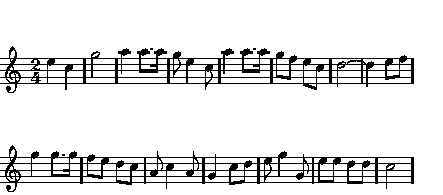
\includegraphics[width=0.8\textwidth]{lilypond}
    \vspace{0.5cm}
  \end{minipage}

  \begin{minipage}[b]{\linewidth}
\begin{lilypond}
\include "header" 
\paper{paper-height = 3.3\cm} 
{
  \key c \major 
  \time 2/4 
  \relative c''
    {
      e4 c g'2 a4 a8. a16 g8 e4 c8 
      a'4 a8. a16 g8 f e c d2~ d4 
      e8 f g4 g8. g16 f8 e d c a c4 a8 g4 
      c8 d e8 g4 g,8 e' e d d c2
    } 
}
\end{lilypond}
  \end{minipage}
  \caption{Intégration de partitions avec Lilypond.}
  \label{fig:lilypond}
\end{figure}
%%%%%%%%%%%%%%%%%%%%%%%%%%%%%%%%%%%%%%%%%%%%%%%%%%%%%%%%%%%%%%%%%%%%%%%%%%%%%%%%

Enfin, pour insérer votre partition \file{sheet.ly} dans une
chanson, utilisez la commande \latexcom{lilypond} le fichier
\ext{sg} adéquat~:

\begin{songbook}
\lilypond{sheet}
\end{songbook}

%------------------------------------------------------------------------------
\subsection{Exemple}
%------------------------------------------------------------------------------

Voici l'exemple complet de la chanson \emph{Sad robot} par
\emph{Pornophonique}\footnote{\byncnd~\url{http://www.jamendo.com/fr/track/81740}}
pouvant être utilisé comme point de départ pour écrire une nouvelle
chanson.

\begin{songbook}
\selectlanguage{english}
\songcolumns{2}
\beginsong{Sad robot}
  [by=Pornophonique,cov=8-bit-lagerfeuer,album=8-bit lagerfeuer]

  \cover
  \gtab{Dm}{XX0231}
  \gtab{F}{1:022100}
  \gtab{C}{X32010}
  \utab{Dm}{2210}
  \utab{F}{2010}
  \utab{C}{0003}

  \lilypond{Sad_robot}

  \begin{verse}
    His \[Dm]steely skin is covered
    By \[F]centuries of dust
    \[C]Once he was a great one
    \[Dm]Now he's dull and rust
  \end{verse}

  \begin{verse*}
    An oily tear he's crying
    Can you feel the pain
    Of the sad, sad robot
    And it's driving him insane
  \end{verse*}

  \begin{verse*}
    He can't turn back time nor history
    So his life became a misery
    He has to face the destiny
    Nobody cares anymore
  \end{verse*}

  \begin{chorus}
    Sad, sad robot
    Sad, sad robot
    Sad, sad robot
    All alone
  \end{chorus}

  \begin{chorus}
    He's a sad, sad robot \rep{3}
    He's so alone
  \end{chorus}

\endsong
\end{songbook}
